\section{Experiments}
\label{sec:experiments}

% DRAFT 2026-11-19, tables plus a few bullets for the author to write out. The setup moved here from the results.
% Sources: decisions.md D6, D8, D10-D12 (supervision/), the campaign plan (supervision/campaign_plan.md, draft 3),
% method.md (code repo, docs/), integration/scenario.py. Only choices that matter for reading the results are
% justified; the rest are settings.
% Run names -> campaign names in the code (integration/run_campaign.py): scale runs = study1 (2024 replays:
% replay/run_points.py on original-2024), phase profiles = study2, moored kept = study5, scene runs = study4a,
% lane revisit runs = study3a, Mid-coast runs = study3b, time-of-day runs = study4b.
% Map: Images/exp_windows_map.pdf, from make_window_map.py (session scratchpad; Natural Earth 10 m land).

\begin{itemize}
    \item One campaign on the code at commit \texttt{b6e1d45} (tag \texttt{report-freeze}), on one laptop (Apple M3, 16~GB, Python 3.11); 4~h 41~min in all. Every setting: Appendix~\ref{app:reproduction}.
    \item Every run saved as one file (settings, truth, labeled measurements, both estimates, per-scan metrics): every number in Chapter~\ref{sec:results} can be recomputed, and every run replayed in the viewer, without running the tracker again.
    \item This chapter: the windows (Section~\ref{sec:exp-windows}), the defaults and the scoring (Section~\ref{sec:exp-scoring}), and the seven sets of runs (Section~\ref{sec:exp-runs}).
\end{itemize}

% =====================================================================
\subsection{Windows}
\label{sec:exp-windows}

\begin{itemize}
    \item Nine windows on the Norwegian AIS day 2025-09-25 (Section~\ref{sec:sim-truth}), of four kinds (Figure~\ref{fig:exp-windows}, Table~\ref{tab:exp-windows}).
    \item Chosen from the data: enough vessels, and no long AIS gaps for the moving vessels, since the truth bridges a gap with a straight line. % source: method.md s2 (named windows): every moving vessel reports at least every 6 min over 100 min of 120 s scans; rejected: Oslofjord (9 h gap), Tampen (3.4 h), Haltenbanken, the Lofoten lanes
    \item Mid-coast is the window for the geometry: of three large candidates it had the most vessels and the fewest long gaps (656--699 vessels per scan, 1\,\% of the moving truth in a gap of more than 60~min). % source: method.md s2; the others: an enlarged North Sea (13 %) and off Troms-Finnmark (a third of the vessels)
\end{itemize}

\begin{figure}[htbp]
    \centering
    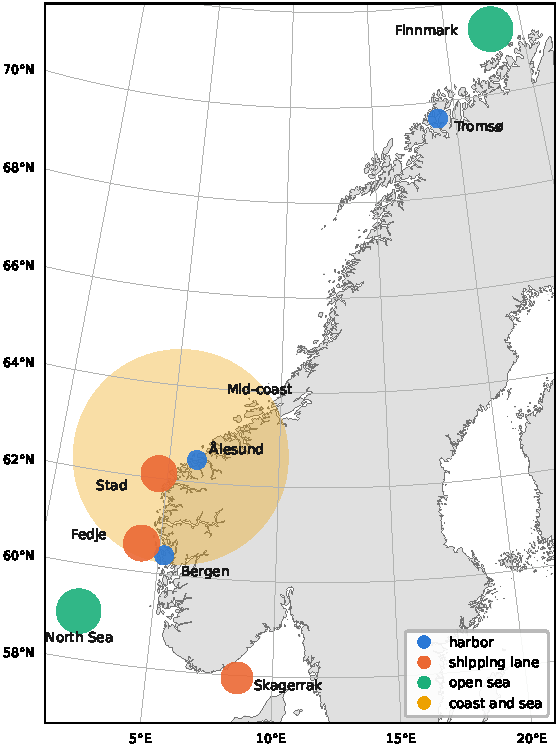
\includegraphics[width=0.55\textwidth]{Images/exp_windows_map.pdf}
    \caption{The nine windows, drawn to scale and colored by kind. Lambert conformal projection; coastline from Natural Earth \TODO{cite Natural Earth}.}
    \label{fig:exp-windows}
\end{figure}

\begin{table}[htbp]
\centering
\caption{The windows on the AIS day 2025-09-25, by kind. Vessels: mean number of moving vessels scored in a scene run (50 scans at 120~s; for Mid-coast, in a Mid-coast run at 300~s).}
\label{tab:exp-windows}
\small
\begin{tabular}{l l r r l r}
\toprule
Kind & Window & Center & Radius [km] & Start (UTC) & Vessels \\
\midrule
Harbor & Bergen & 60.40\,N 5.22\,E & 20 & 06:00 & 51 \\
 & Ålesund & 62.47\,N 6.25\,E & 20 & 06:00 & 37 \\
 & Tromsø & 69.65\,N 18.95\,E & 20 & 06:00 & 12 \\
\addlinespace
Shipping lane & Skagerrak & 57.95\,N 8.60\,E & 35 & 06:00 & 17 \\
 & Fedje & 60.60\,N 4.20\,E & 40 & 06:00 & 21 \\
 & Stad & 62.10\,N 4.60\,E & 40 & 10:00 & 27 \\
\addlinespace
Open sea & North Sea & 59.00\,N 2.00\,E & 50 & 14:00 & 19 \\
 & Finnmark & 71.35\,N 23.00\,E & 50 & 06:00 & 4 \\
\addlinespace
Coast and sea & Mid-coast & 62.50\,N 5.50\,E & 250 & 06:00 & 769 \\
\bottomrule
\end{tabular}
\end{table}

% =====================================================================
\subsection{Defaults and scoring}
\label{sec:exp-scoring}
\label{sec:exp-defaults}

\begin{table}[htbp]
\centering
\caption{Defaults of every run unless Table~\ref{tab:exp-runs} says otherwise, and how runs are scored.}
\label{tab:exp-defaults}
\small
\begin{tabularx}{\textwidth}{l l X}
\toprule
Setting & Value & Note \\
\midrule
Sensor & EO, $\sigma = 300$~m, $P_{\mathrm{D}} = 0.9$ & Section~\ref{sec:sim-sensors} \\
Clutter & $10^{-9}$~m$^{-2}$ & At $10^{-7}$ the stock tracker crashed at the proof-of-concept size \\ % source: method.md s2
Scans & 50 at 120~s & \\
Tracker & n-vector, clustered, recycling & Parameters: Section~\ref{sec:impl-parameters} \\
Moored vessels & Left out & Within 100~m of the median position at every scan; see below \\
Seeds & 5 (0--4) & A seed changes noise, missed detections and clutter, not the truth \\
Estimates & Online and lagged & Lagged: $L = 5$ scans later, smoothed; see below \\
Warm-up & 10 scans & 5 in the lane revisit and Mid-coast runs \\
\addlinespace
Accuracy & GOSPA, $p = 2$, $\alpha = 2$, $c = 1000$~m & Great-circle distances \TODO{cite Rahmathullah et al.\ 2017}. Missed and false as shares of the vessel-scans, localization as the RMSE of the matched pairs. Compares runs on the same scene only \\
Continuity & Table~\ref{tab:exp-continuity} & Rates per 1000 vessel-scans \\
Run time & Tracker step per scan & Wall clock, without scoring. Scale runs and profiles one job at a time, the rest three in parallel ($\pm 15$\,\% \TODO{source: method.md s5.2}) \\
\bottomrule
\end{tabularx}
\end{table}

\begin{table}[htbp]
\centering
\caption{Continuity metrics. Every scan, each vessel keeps the track it was matched to in the previous scan while that track is within $c$; the rest are matched by GOSPA's assignment (as in CLEAR-MOT \TODO{cite Bernardin \& Stiefelhagen 2008}).}
\label{tab:exp-continuity}
\small
\begin{tabularx}{\textwidth}{l X}
\toprule
Metric & Definition \\
\midrule
ID switch & The vessel's track differs from its last matched track \\
Fragmentation & The vessel is matched, then unmatched, then matched again, whatever the track \\
Coverage & Share of a vessel's scans in view in which it is matched to a track \\
Tracks per vessel & Number of different tracks matched to a vessel \\
Purity & Share of a track's measurement updates from its majority vessel (from the measurement labels) \\
\bottomrule
\end{tabularx}
\end{table}

\begin{itemize}
    \item Moored vessels are left out because moored vessels side by side dominate the scores, and harbor tracking is later work; agreed with the supervisors. A position rule, since only about 40\,\% of moored vessels report their status in AIS. What the filter changes is itself a result (Section~\ref{sec:res-moored}). % source: D6; method.md s2
    \item Continuity is scored apart from GOSPA, which does not see whether a vessel keeps its track. The sticky matching keeps toggles between vessels closer than $\sigma$ from counting as switches. % source: D10
    \item Lagged estimate: each track followed back $L = 5$ scans along its history, reported only if it had a detection in that interval, and smoothed (Rauch-Tung-Striebel). Later scans settle associations, and tracks that coast after their vessel has left are dropped. $L$ is in scans at every revisit time: 10~min late at 120~s, 75~min at 900~s \TODO{the definition may belong in Section~\ref{sec:impl-estimation}}. % source: D8, D11; method.md s4, s5.4 (gain flat from L = 3)
\end{itemize}

% =====================================================================
\subsection{Sets of runs}
\label{sec:exp-runs}

\begin{table}[htbp]
\centering
\caption{The sets of runs, in the order of Chapter~\ref{sec:results}. Fixed: settings that differ from Table~\ref{tab:exp-defaults}. Seeds: per setting. Runs: tracker runs; the scale runs also replay the 2024 code at 9 points. Results: section of Chapter~\ref{sec:results}.}
\label{tab:exp-runs}
\footnotesize
\setlength{\tabcolsep}{4pt}
\begin{tabularx}{\textwidth}{>{\raggedright\arraybackslash}p{1.6cm} >{\raggedright\arraybackslash}X >{\raggedright\arraybackslash}X >{\raggedright\arraybackslash}X r r l}
\toprule
Runs & Question & Varies & Fixed & Seeds & Runs & Results \\
\midrule
Scale runs & RQ1: what each change to the code buys in run time and accuracy & Radius 12--200~km at $10^{-9}$~m$^{-2}$; 50 and 100~km also at $10^{-8}$ and $10^{-7}$; code version O, S, C, R (Table~\ref{tab:exp-versions}) & Bergen center; 30 scans; single plane; online only; stopped at 60~min projected or 10~min per scan & 1 & 28 + 9 & \ref{sec:res-scale} \\
\addlinespace
Phase profiles & RQ1: which phases take the time & The scale runs' points (R); C at 50~km, $10^{-8}$ and $10^{-7}$; S at 50~km, $10^{-9}$ & As the scale runs; 12 scans; phase timers & 1 & 13 & \ref{sec:res-phases} \\
\addlinespace
Moored kept & Is it right to leave the moored vessels out? & Moored vessels kept & Bergen, Ålesund, Stad & 5 & 15 & \ref{sec:res-moored} \\
\addlinespace
Scene runs & RQ3: usable track histories in each kind of scene? Does the lagged estimate help? & The eight windows & -- & 5 & 40 & \ref{sec:res-estimates}, \ref{sec:res-scenes} \\
\addlinespace
Lane revisit runs & RQ3: how the tracker degrades with revisit time. RQ2: does the geometry matter there? & Revisit 120, 300, 600, 900~s & Skagerrak, Stad; 240~min; both geometries & 5 & 40 & \ref{sec:res-geometry}, \ref{sec:res-revisit} \\
\addlinespace
Mid-coast runs & RQ2: where the single plane starts to matter. RQ3 on a large window & Revisit 300, 900, 1800~s & Mid-coast; 8~h; both geometries & 3 & 9 & \ref{sec:res-geometry}, \ref{sec:res-revisit} \\
\addlinespace
Time-of-day runs & RQ3: do the scores follow the traffic over the day? Cases to look at & Start 00, 04, 08, 12, 16, 20~UTC & -- & 1 & 48 & \ref{sec:res-time-of-day} \\
\bottomrule
\end{tabularx}
\end{table}

\begin{table}[htbp]
\centering
\caption{The code versions of the scale runs; each adds one change.}
\label{tab:exp-versions}
\small
\begin{tabularx}{\textwidth}{l X}
\toprule
Version & Change \\
\midrule
O & The 2024 implementation \cite{ais_imm_pmbm} with two one-line fixes so that it runs on today's data; replayed on the same measurements \\
S & The speed-ups that leave the results unchanged (Appendix~\ref{app:speedups}); still one list of global hypotheses \\
C & Clustering (Section~\ref{sec:impl-clustering}), without recycling \\
R & Recycling (Section~\ref{sec:impl-recycling}): the tracker of every other run \\
\bottomrule
\end{tabularx}
\end{table}

\begin{itemize}
    \item Scale runs:
    \begin{itemize}
        \item around Bergen on the Norwegian day, since the AIS files of the proof-of-concept window cover only 58--63\,N, 4.5--7.5\,E; % source: method.md s2
        \item up to 200~km, since with the moored vessels left out a radius holds far fewer vessels (about 80\,\% are moored); 200~km gives about 425 moving vessels; % source: method.md s2; Table tab:res-ladder
        \item in the single plane, since the 2024 code has no n-vector geometry; % source: method.md s1
        \item the time limits keep the campaign within a night: without them, the stock code at 100~km and $10^{-7}$~m$^{-2}$ alone would take about 8~h. S and C are not run there (3300 measurements per scan) \TODO{source: method.md s5.2}. % source: D12
    \end{itemize}
    \item Lane revisit runs: the same 240~min at every revisit time, so every point sees the same vessels; a warm-up of 5 scans, since confirming a track takes detections, not time, and 900~s gives only 16 scans. % source: D11; campaign plan, study 3a
    \item Mid-coast runs: by the error budget (Section~\ref{sec:nvector-error}) the single plane's error needs hundreds of km and long gaps between scans; 3 seeds, since the comparison is paired on the same measurements. % source: D11, D12; method.md s5.1
    \item Time-of-day runs: start times instead of seeds, to cover more of the AIS data. Only the default start times were checked for AIS gaps. % source: D11; campaign plan, study 4b
\end{itemize}
